\documentclass[useAMS,usenatbib]{mn2e}
\usepackage{graphicx}
\newcommand{\figpath}{./Figs/}

%--------------------------------------------------------------------
\title[Geometrically thin acrretion disk around white dwarfs and quark stars]{Geometrically thin acrretion disk around white dwarfs and quark stars}
\author[B. Mishra, W. Klu\'zniak and B. Vaidya]{B. Mishra$^{1}$\thanks{E-mail:
mbhupe@camk.edu.pl}, W. Klu\'zniak$^{1}$, B. Vaidya$^{2}$\\
$^{1}$Copernicus Astronomical Center, Bartycka 18, Warsaw,00-716, Poland\\
$^{2}$University of Leeds, Leeds LS2 9JT, United Kingdom}
%%%%%%%%%%%%%%%%%%%%%%%%%%%%%%%%%%%%%%%%%%%%%%%%%%%%%%%%%%%%%%%%%%%%%%
\begin{document}
\date{Accepted *** Received 000}
\pagerange{\pageref{firstpage}--\pageref{lastpage}} \pubyear{2014}
\maketitle
\label{firstpage}
%--------------------------------------------------------------------
\begin{abstract}
We studied semi-analytically and numerically the geometrically thin and optically thick accretion disk around rapidly rotating quark stars and white dwarfs using potential for Maclaurin spheroid. The main interest is to investigate the inner region of the so called $\alpha$-disk. We found that the change in eccentricity of the compact object influence the spectra emitted from the accretion disk. This can be observational evidence for the existance of the quark stars. Analytical calculations are mainly done in the radiation pressure dominated region of the accretion disk. The numerical work has been carried out to see the time evolution of the accretion disk around quark stars and white dwarfs using the same potential for Maclaurin spheroids. We showed that if the eccentricity of the object is high the matter will diffuse slowly and advect rapidly during its evolution. This gives a clue that how spin up or spin down can change the time evolution of the accretion disk using a very simple Newtonian approach.  
\end{abstract}
%--------------------------------------------------------------------
\begin{keywords}
Maclaurin spheroids, white dwarfs, quark stars, accretion disk
\end{keywords}
%--------------------------------------------------------------------
\section{Introduction}
Accretion disk has remained a challenging problem mainly in the context of its viscosity prescription and radiative processes. The best known models for describing the accretion disk were proposed by Shakura and Sunyaev(1973) (SS73 here after), Novikov and Thorne (1973) and Lynden-Bell and Pringle(1974). The underling assumption behind all these models was a geometrically thin accretion disk because of assumption that accreting gas is cool as compare to the local virial temperature. There was also an assumption of equilibrium between viscous energy generation inside the disk and radiative cooling from the surface of the disk, where radiative cooling was computed with an assumption that disk is optically thick in the vertical direction. Although these models has been intensively used to describe the accretion disk around different accreting sources however these models are more suitable for accreting sources like white dwarfs and neutron stars. These models had less successful implications directly to sources like black holes where gravity is much higher and one has to take into account the consequences of Lightman-Eardley instability. 

In the seminal paper SS73 analytically solved the accretion disk model assuming that the source of viscosity is turbulence present in the accretion disk. Till date the exact mechanism of existing viscosity in the accretion disk is not clear. Ballbus Hawley 1991 considered magneto-rotational instability (MRI) to explain the source of viscosity, which fulfills some of the criterion for viscosity in the accretion disk. We shall consider a simple constant $\alpha$ viscosity model to study the accretion disk around quark-stars and white dwarfs without considering effect of magnetic field.

SS73 considered Newtonian potential around spherically symmetric black holes. First time we are considering the accretion disk around an accreting source which has spheroidal shape rather than spherical. We shall use Maclaurin spheroid potential for a constant density and mass of the central accreting object. We investigated that how the non-keplerian angular velocity will change the dynamics of the accreting matter into the source. Our goal is to study mainly inner region of the accretion disk where the multipole effects of chosen Maclaurin spheroid potential dominates. We followed the same model as SS73 just by changing the potential of the central object for Maclaurin spheroid. We used same constant $\alpha$ viscosity prescription to proceed analytic and numerical work. We did the analytical calculation of various parameters of the accretion in all three regions but we shall focus only in the inner region which is also radiation pressure dominated region as per choice of the SS73 model. 

We took into account the main property of the choice of such a potential which corresponds to innermost stable circular orbit (ISCO) even in Newtonian dynamics (Kluzniak et al 13). We chose a constant density and mass quark star and assumed that it is rotating very rapidly. Since during rapid rotation it can change its eccentricity and so semi-major axis of the star. Either eccentricity can decrease or increase, depending on it the semi-major axis will decrease or increase. In Kluzniak et al 13, it has been shown that if the eccentricity is less than a critical value of $e_c = 0.8345$, the ISCO will lie on the equator of the acreting source but if it is higher than this critical value it will be detached from the surface of the star. Keeping this change in ISCO we assumed the cases where eccentricity is less than critical limit. We see a change in inner radii of the accretion disk with change in eccentricity because the semi-major axis of the accreting quark star is changing. This change in the inner radii of the accretion disk due to change in eccentricity will clearly change the calculated parameters like surface density, height and emitted spectra of the accretion disk. However there is very minor change in the steady state results so we also investigated the non-stationary accretion disk.

We studied the time evolution of the accretion disk around quark star by solving the diffusion equation for the matter around accreting source. We again assumed the same potential as in steady disk study. In numerical work we studied that how change in eccentricity will change the time evolution of the accretion disk. We shall describe in the results that higher the eccentricity lower the diffusion of matter and lower the eccentricity higher the diffusion of the matter. In all cases we made a cross check to our results by taking limit that $e\rightarrow0$, this will assure us that our analytical and numerical results are consistent with the existing results.

The article is organized in the following manner. In \S 2 we described physical model of accretion disk which covers steady thin disk and also numerical study of the time evolution of the accretion disk. \S3 is devoted for describing all the results we obtained analytically and numerically. In \S4 we shall discuss all the results described in \S3 and we shall conclude in \S5 with some real future applications of our accretion model around quark stars and white dwarfs.  
%-----------------------------------------------------------------------
\section{Physical Model}
\subsection{Maclaurian Spheroid}
\begin{itemize}
\item Describe in very brief the basics and how $\Omega$ is obtained
  and re-draw the plot that is in your supervisor paper. 
\end{itemize}
In general the accretion disk has been studied for the potential due to spherically symmetric objects which corresponds to Keplerian velocity. We are using potential for the Maclaurin spheroids which corresponds to angular velocity which is non-Keplerian in the inner region of the disk. The detailed description of the angular velocity has been studied by Kluzniak et al 2013. The angular velocity on the equatorial plane at a radial distance $r$ from the center of a spheroidal quark star or white dwarf with eccentricity $e$ and semi-major axis $a$ is given by Eqn.~\ref{omega}. The non-Keplerian angular velocity reduces to Keplerian in two extreme cases one for $e\rightarrow 0$ and other for $r\rightarrow \infty$. This is also one reason we are more interested in the inner region of the accretion disk, which is also radiation pressure dominated region according to SS73 model.
\begin{figure}
\centering
\includegraphics[width=1\columnwidth]{\figpath/angular.eps}
\caption{Angular velocity distribution for chosen Maclaurin spheroid potential. The important point to notice in the figure is the inner radii, which varies with eccentricity. This corresponds to different disk inner radii for different values of eccentricity $e$ and corresponding semi-major axis $a$}
\label{fig:steadyplt1}
\end{figure}
\begin{equation}
\Omega ^2 \left(R\right)= 2\pi G\rho_* \frac{(1-e^2)^{1/2}}{e^3}\left[\gamma - \cos \gamma \sin\gamma \right]
\label{omega}
\end{equation}  
where $\gamma = \arcsin (\frac{a e}{r})$ and $\rho * = const$ is density of star. Now we have angular velocity of the matter for chosen potential, next goal is to adopt SS73 disk model and redo whole calculations for angular velocity calculated in Eqn.~\ref{omega}.
%-------------------------------------------------------------------
\subsection{Steady thin accretion disk}
\begin{itemize}
\item List all the equations that you have used and what modification
  you have done for e.g., you have used $\Omega$ corresponding to
  MacLaurian spheroid. 
\item Say that formulae depends on M, Mdot, $\alpha$, r and
  eccentricity and give the values of choices made for them. 
  Explicit formulae and quantities shall be discussed in results
  section.
\end{itemize}
Now we can use Eqn.~\ref{omega} and follow exactly same steps as SS73, to calculate analytically at three different regions of the accretion disk. Our main concern here will be inner region, which is radiation pressure dominated region. We shall present all the equations and algebraic parameters in the second and third regions also but since we know that at large radii our results reduce to Newtonian results we shall investigate inner region only in detail.
%----------------------------------------------------------------
\subsubsection{Radiation pressure dominated region}
SS73 considered three different regions in the accretion disk, the inner one is radiation pressure dominated where in the interaction of matter and radiation electron scattering on free electrons has dominating contribution. Fig.~\ref{prpg} confirms that our results are in the region where radiation pressure dominates over the gas pressure. We shall directly write the final form of the algebraic equations to calculate the different parameters in the different regions of the disk (SS73).
\begin{equation}
z_0(r) = \frac{\sigma\rho_0\dot{M}k_1\left(p_1^{1/2}r^2 - p_2^{1/2}R_0^2\right)(ae)^3}{8\pi r^5 c \rho \Omega^2\cos\gamma(\gamma - \sin\gamma\cos\gamma)^{1/2}}.
\end{equation}
\begin{equation}
\Sigma(r) = \frac{32\pi c^2\rho^2 r^8 \cos^2{\gamma}(\gamma - \sin\gamma\cos\gamma)^2}{\alpha\sigma^2\rho_0^2 k_1^{1/2}(ae)^6\dot{M}\left(p_1^{1/2}r^2 - p_2^{1/2}R_0^2\right)}.
\end{equation}
\begin{equation}
\varepsilon(r) = \frac{6 r^3 c \cos\gamma(\gamma - \sin\gamma\cos\gamma)^{3/2}k_1^{1/2}}{\alpha\sigma (ae)^3}
\end{equation}
\begin{equation}
T(r) = \frac{6r^3 c \cos\gamma (\gamma - \sin\gamma\cos\gamma)^{3/2}k_1^{1/2}}{b^{1/4}\alpha\sigma (ae)^3}
\end{equation}
\begin{equation}
\tau (r) = \sqrt{\sigma_T(0.11 T^{-7/2}n)}\Sigma(r)
\end{equation}
\begin{equation}
n(r) = \frac{\Sigma(r)}{2mpz_0(r)}
\end{equation}
\begin{equation}
v_r(r) = \frac{\dot{M}}{2\pi\Sigma r}
\end{equation}
where, 
\begin{equation} 
\gamma = \arcsin(\frac{ae}{r}) 
\end{equation}
\begin{equation}
\gamma_0 = \arcsin(\frac{ae}{R_0})
\end{equation}
\begin{equation}
p_1 = (\gamma - \sin\gamma\cos\gamma)
\end{equation}
\begin{equation}
p_2 = (\gamma_0 - \sin\gamma_0\cos\gamma_0)
\end{equation}
$\dot{M}$ is mass accretion rate, $z_0(r)$ is half thickness of the disk, $\Sigma(r)$ is the radial distribution of surface density, $\varepsilon(r)$ is radial distribution of energy density, $T(r)$ is radial distribution of the temperature, $\tau(r)$ is optical thickness, $n(r)$ is the number density and $v_r$ is the radial velocity of the matter in the steady thin accretion disk.
%------------------------------------------------------------------
\subsubsection{Gas pressure dominated region, electron scattering}
This is the middle region of the accretion disk in which gas pressure dominates over the radiation pressure $(P_g >> P_r)$. In this region also similar to inner region electron scattering gives main contribution to opacity. The sound speed in this region is given by $v^2_s = \frac{kT}{m_p}$. 
\begin{eqnarray}
\Sigma(r) = \left(\frac{\dot{M}}{\pi}\right)^{3/5}\left(\frac{m_p}{\alpha k}\right)^{4/5}\left(\frac{bc}{3\sigma}\right)^{1/5}r^{-7/5} 
\end{eqnarray}
$$ \left(\Omega r^2 -\Omega_0 R_0^2\right)^{3/5}\left(\frac{d\Omega}{dr}\right)^{-1/5}$$
\begin{equation}
T(r) = 0.707106 \pi^{-3/20}\left(\frac{3\sigma}{bc}\right)^{1/5}\dot{M}^{2/5}r^{-7/20}
\end{equation}
$$ \left(\Omega r^2 - \Omega(R_0) R_0^2\right)^{2/5}\left(\frac{m_p}{\alpha k}\frac{d\Omega}{dr}\right)^{1/5}$$
\begin{equation}
z_0(r) = \sqrt{\frac{k T}{m_p\Omega^2}}
\end{equation}
\begin{equation}
n(r) = \frac{\Sigma(r)}{2m_p z_0}
\end{equation}
\begin{equation}
\tau(r) = \sqrt{\sigma_T \sigma_{ff}}\Sigma
\end{equation}
\begin{equation}
v_r = \frac{\dot{M}}{2\pi\Sigma(r) r}
\end{equation}
where, $\Omega$ is given by Eqn.1, $\Sigma(r)$ is the height integrated surface density, $T(r)$ is the temperature, $z_0(r)$ is the half thickness of the disk, $n(r)$ is the number density, $\tau(r)$ is the optical thickness and $v_r$ is the radial velocity. $\Omega$ is the angular velocity, $\sigma$ is opacity, $c$ is speed of light, $\alpha$ is angular momentum transportation factor, $m_p$ is the mass of proton, $\sigma_T$ is Thompson cross-section and $\sigma_{ff}$ is opacity due to free free absorption.
%--------------------------------------------------------------------
\subsubsection{Gas pressure dominated region, free-free absorption}
In this region similar to gas pressure dominated region $P_g > P_r$ but the opacity is determined by free-free absorption. Sound speed is defined similar to middle region (gas pressure dominated region with electron scattering) $v^2_s = \frac{kT}{m_p}$.
\begin{equation}
\Sigma (r) = \left(\frac{m_p}{(2\pi\alpha k)^{4/5}}\right)\left(\frac{32\pi R bc \dot{M}^7\left(\Omega r^2 - \Omega_0 R_0^2\right)}{3\Omega\frac{d\Omega}{dr}}\right)^{1/10}
\end{equation}
\begin{equation}
T(r) = \left(\frac{3Q \Sigma^{1/2}\Omega}{2 m_p^{1/2}}\right)^{1/8}
\end{equation}
\begin{equation}
z_0(r) = \sqrt{\frac{k T(r)}{m_p\Omega^2}}
\end{equation}
\begin{equation}
n(r) = \frac{\Sigma(r)}{2m_p z_0(r)}
\end{equation}
\begin{equation}
\tau = \sigma_{ff}\Sigma(r)
\end{equation}
\begin{equation}
v_r = \frac{\dot{M}}{2\pi\Sigma(r) r}
\end{equation}
where 
\begin{equation}
Q = -\frac{\dot{M}\left(\Omega r^2 - \Omega(R_0)R_0^2\right)}{4\pi r}\frac{d\Omega}{dr}.
\end{equation}
is the energy flux radiated from unit surface of disk in unit time and rest of the parameters defined above have the same notation as in the inner region and middle region of the accretion disk.
%---------------------------------------------------------------------
\subsection{Non-stationary accretion disk}
\begin{itemize}
\item List formulae and refer the paper that we have been using for
  evolution of Surface density. 
\end{itemize}
The disk may not be stationary due to viscous forces acting to transport the angular momentum and cause the accretion of the matter. Here we numerically studied the time evolution of the thin accretion disk around quark stars. We shall integrate numerically the diffusion equation with constant viscosity. We used Crank-Nicolson method which is re-described in Brensteil et al 2010 to solve the linear diffusion equation. One can also solve the same equation using Green's function but the expressions in case of Maclaurin spheroid potential are not trivial to handle analytically. For the potential we adapted from Maclaurin spheroids gives the different angular velocity profile so we shall write the diffusion equation in terms of angular velocity. This set of equations can be fed with any form of potential or angular velocity.
\begin{equation}
\frac{\partial\Sigma}{\partial t} = -\frac{1}{r}\frac{\partial}{\partial r}\left[\frac{1}{2\pi(r^2\Omega)^\prime}\frac{\partial G}{\partial r}\right]
\label{diffusion}
\end{equation}
\begin{equation}
v_r = \frac{1}{2\pi}\frac{\frac{\partial G}{\partial r}}{r\Sigma (r^2\Omega)^\prime}
\label{velocity}
\end{equation}
where,
\begin{equation}
G(r,t) = 2\pi r\nu\Sigma r^2 \Omega^\prime 
\end{equation}
is the torque exerted by the outer ring to inner ring in the accretion disk or $-G(r,t)$ is torque exerted by the inner ring to the outer ring. Now if we choose the Keplerian angular velocity the above equations will reduce to standard diffusion equation used for study of disk evolution by various models based on $\alpha$-disk models.
\begin{equation}
\frac{\partial\Sigma}{\partial t} = \frac{3}{r}\frac{\partial}{\partial r}\left[r^{1/2}\frac{\partial}{\partial r}\left(\nu\Sigma r^{1/2}\right)\right]
\end{equation}
\begin{equation}
v_r = -\frac{3}{\Sigma r^{1/2}}\frac{\partial}{\partial r}\left(\nu\Sigma r^{1/2}\right)
\end{equation}
where $\Sigma$ is the surface density, $\nu$ is kinematic viscosity. Now using Eqn.~\ref{omega}, Eqn.~\ref{diffusion} and Eqn.~\ref{velocity} we shall compute the time evolution of the accretion disk for different eccentricities $e$ of the quark star. Depending on eccentricity $e$, either matter can be diffused rapidly or slowly. If the eccentricity is high matter will diffuse very slowly as compare to low eccentricity, which we shall describe in the results.
%----------------------------------------------------------------------
\section{Results}
\subsection{Steady state disk}
In this section we shall use Eqn.2 to Eqn.8 to investigate the inner region of the accretion disk. Fig.2 shows the variation of the height $z_0(r)$, surface density $\Sigma(r)$, temperature $T(r)$ and radial velocity $v_r(r)$. As in standard SS 1973 disk the thickness $z_0(r)$ is directly proportional to mass-accretion rate $\dot{M}$, higher the accretion rate will correspond thicker accretion disk. Here we keep accretion rate fixed at $\dot{M} = 10^{13} g/s$, density of the star at $10^15 g/cm^3$ and changed the eccentricity $e$ to see the effect on the thickness of the accretion disk. We see from upper left panel of Fig.~\ref{steadyplt1} a clear difference in the half thickness of the accretion disk for eccentricities $e =0.1$, $e = 0.2$ and $e = 0.8345$. The inner radii of the disk is a function of eccentricity which cause a variation in the inner radii of the accretion disk. There is important difference between potential for Maclaurin spheroids and spherical object. The radius $R$ of the Maclaurin spheroid changes with eccentricity and this corresponds to semi-major axis of the star of constant density and mass. 
\begin{equation}
a = \frac{R}{(1 - e^2)^{1/6}}
\end{equation}
The maximum of radial epicyclic frequency lies at $r = \sqrt{2}ae$ for spheroid eccentricities $e>1/\sqrt{2}$ but it vanishes for $e_c = 0.83458318$ at the equator of the star (Kluzniak et al 2013). If we still increase the eccentricity further $e>e_c$, the innermost stable circular orbit (ISCO) will be separated from the equator of star and it will be at $r_{ms} = 1.198203ae$ (Kluzniak et al 13). This is the reason we chose $e = 0.8345$ in Fig.~\ref{steadyplt1}. So we always keep the inner radius of the accretion disk at variable semi-major axis of the quark star. One can increase the eccentricity further to investigate the accretion disk for which the inner radii does not lie at the surface of the star. Right upper panel in Fig.~\ref{steadyplt1} shows the variation of the surface density $\Sigma(r)$ with radial distance. For higher eccentricity the surface density is higher as compare to low eccentricity ??. Lower left panel shows the variation of temperature in the inner region of the accretion disk. Higher eccentricity corresponds to low temperature due to higher disk thickness and surface density ??. Right lower panel shows the radial velocity of the accreting matter. Since radial velocity is inversely proportional to surface density it has lower value for higher eccentricities, we also see clearly from radial velocity profile that close to inner radii of the accretion disk radial velocity is almost speed of light. From Fig.~\ref{prpg} we can make sure that the region we are studying is under the assumption of radiation pressure domination over gas pressure.

The most important parameter for observational interest is emitted spectra from the accretion disk. Emitted spectra directly represents the size of the accretion disk. Fig.~\ref{spectra} shows the emitted spectra from the accretion disk. Since the computed spectra is independent of any region specified above we can choose an arbitrary outer radii of the accretion disk to see the behavior of the emitted spectra. Here accretion disk we assumed optically very thick therefore we can apply black body spectra to calculate the spectra emitted from the accretion disk. The next subsection \S3.2 is devoted for the study of the spectra emitted from the disk.
\begin{figure}
\centering
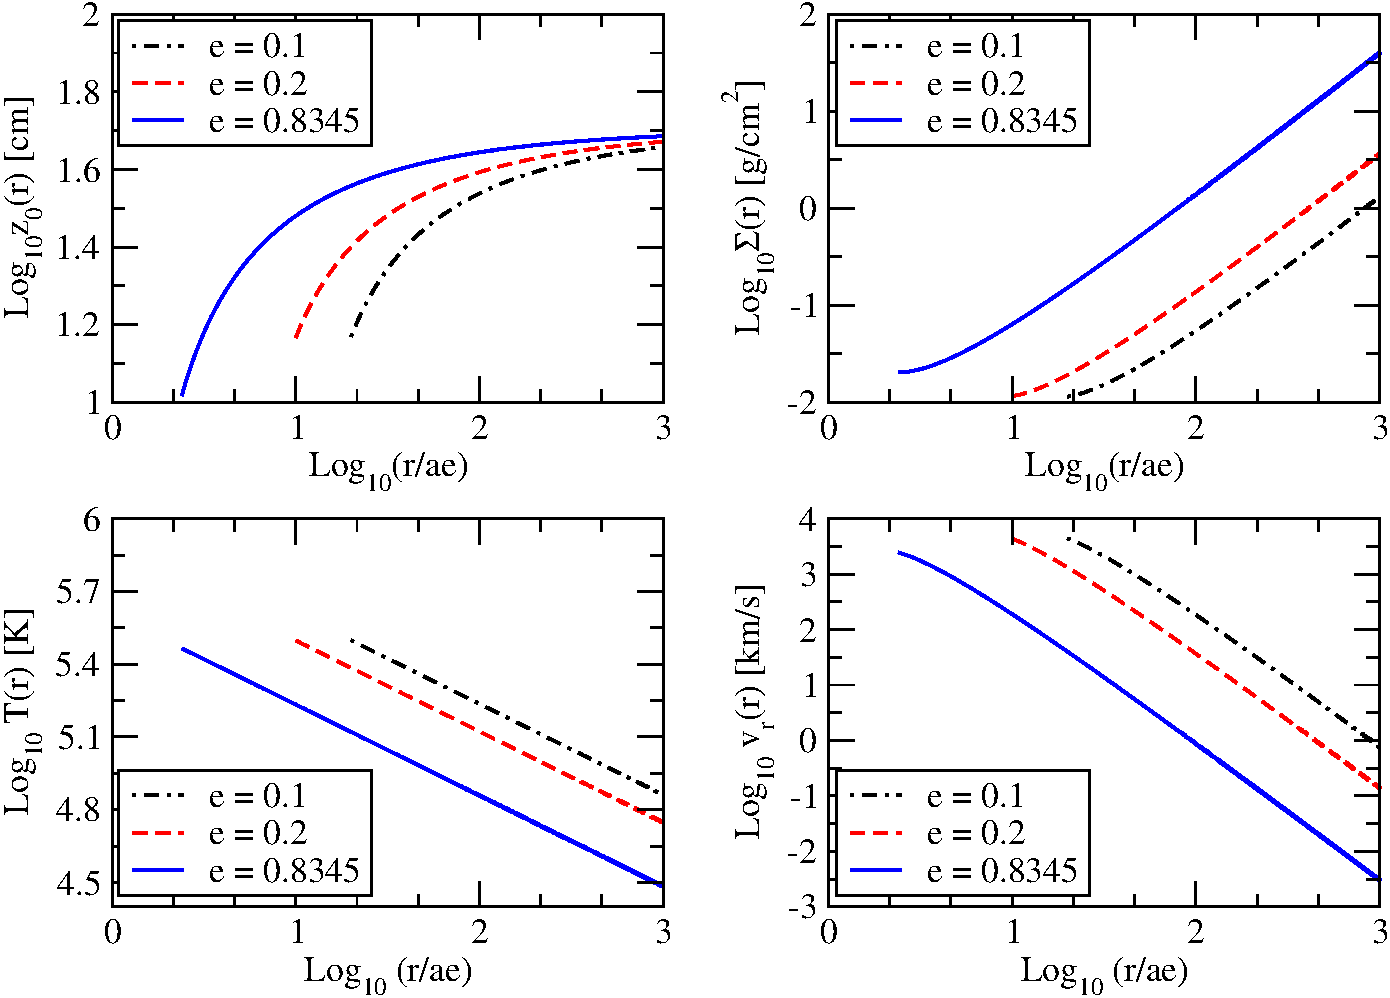
\includegraphics[width=1\columnwidth]{\figpath/multiplot_rho_alpha0001.pdf}
\caption{Multiplot of height, surface density, temperature and radial velocity variation with radial distance from the center of the star }
\label{steadyplt1}
\end{figure}

\begin{itemize}
\item describe the multi plots (fig~\ref{fig:steadyplt1}) for each quantity : its value, its
  profile and dependence on eccentricity.
\item Make a table which gives quantitive values.  
\end{itemize}
%-----------------------------------------------------------------------
\subsection{Disk thermodynamics and Spectra}
\begin{itemize}
\item Show that values of T obtained above give Prad $>$ Pgas. 
\item Also show that the disk is optically thick.
\item Finally describe the spectra and state its dependence on
  eccentricity. (Explain the reason in discussion).
\end{itemize}
Using angular velocity from Eqn.~\ref{omega} and equating the dissipation rate per unit area to the blackbody flux we computed temperature of the accretion disk.
\begin{equation}
T(r) = \left[\frac{-\Omega\frac{d\Omega}{dr}T_1}{4\pi\sigma}\right]^{1/4}
\end{equation}
where $T_1$ is defined as
\begin{equation}
T_1 = 1 - \frac{\Omega(a)a^2}{\Omega(r)r^2}
\label{T1}
\end{equation}
Now using a very crude approximation we can approximate the emitted spectra in cgs units by
\begin{equation}
I(\nu) = B_{\nu}[T(r)] = \frac{2h\nu^3}{c^2(e^{h\nu/kT(r)} -1)}
\end{equation}
using Eqn.~\ref{T1} we computed flux emitted from accretion disk by integrating over the whole disk.
\begin{equation}
F(\nu) = \frac{2\pi}{D^2}\int^{R_{out}}_{R_{in}}I(\nu)rdr
\label{flux}
\end{equation}
the numerical integration of Eqn.~\ref{flux} gives emitted spectra from the disk (Fig.~\ref{spectra}). We chose outer radii $R_{out} = 10a$ and $R_{out} = 100a$ in Fig.~\ref{spectra} to see the behavior of the emitted spectra for different eccentricity of the quark star. We see clearly that a change in outer radii $R_{out}$ of the disk changes the emitted spectra at lower frequency while change in eccentricity which corresponds to change in inner radii $R_{in}$ of the accretion disk causes a very minor change in emitted spectra at high frequency. There is also a very minor difference across the whole range of the emitted spectra for different eccentricities. At $h\nu/kT = 10$ curves for $e = 0.83$, $R_{out} = 100a$ and $e = 0.5$, $R_{out} = 10a$ have the same value of emitted flux. Therefore a change in eccentricity of the accreting source do not has a significant change in the emitted spectra of the accretion disk.
\begin{figure}
\centering
\includegraphics[width=1\columnwidth]{\figpath/pradpgas.eps}
\caption{Plot shows the the inner region of investigation in which we assumed that radiation pressure dominates over gas pressure}
\label{prpg}
\end{figure}
\begin{figure}
\centering
\includegraphics[width=1\columnwidth]{\figpath/spectra.eps}
\caption{Plot shows the the inner region of investigation in which we assumed that radiation pressure dominates over gas pressure}
\label{spectra}
\end{figure}
%-----------------------------------------------------------------------
\subsection{Evolution of surface density}
\begin{itemize}
\item Show the plot of evolution of a ring of matter for a particular high
  eccentricity and describe it. Specially the skewed profile for
  higher eccentricity. 
\item Show that at low eccentricity it approaches the $\alpha$-disk
  solution. Here also describe the plot which shows the evolution with
  different eccentricity. 
\end{itemize}
We shall use the physical model of \S2.3 for non-stationary disk and numerically solve Eqn.~\ref{diffusion} and Eqn.~\ref{velocity} to study the time evolution of the accretion disk in case of non-spherical chosen potential of Maclaurin spheroids. We see from Fig.~\ref{omega} that for higher values of the eccentricity of the accreting quark stars the angular velocity $\omega(r)$ is lower as compare to $\omega(r)$ for lower eccentricity. This also corresponds that if the eccentricity is higher there will be less friction between neighboring rings of the matter in the accretion disk and this will imply slow angular momentum transport outwards and low diffusion of the matter into the accreting source. We chose a Gaussian ring of matter and put it at a radial distance of $r/a = 1.5$ as the initial condition to solve the diffusion equation Eqn.~\ref{diffusion}. In Fig.~\ref{evolve} we plotted the time evolution of surface density scaled with initial surface density. The horizontal axis corresponds to radial distance scaled with semi-major axis of the quark-star. Left panel in Fig.~\ref{evolve} shows the time evolution of the accretion disk for an accreting source with eccentricity $e = 0.83$ and the right panel of Fig.~\ref{evolve} shows the time evolution for eccentricity $e = 0.5$. 

In all the time evolution plots the time is in viscous time scale and the kinematic viscosity coefficient $\nu = 0.01$. We see a clear difference in time evolution of the initial Gaussian ring of matter for different eccentricity in Fig.\ref{evolve}, higher the eccentricity lower the diffusion of the matter and lower the eccentricity higher the diffusion of the matter. Fig.~\ref{evolve1e-4} shows the behavior of the ring of matter we put for very low values of eccentricities. Left panel in Fig.~\ref{evolve1e-4} shows the time evolution of the ring for eccentricity $e = 0.0001$ and the right panel again same as right panel of Fig.~\ref{evolve} for eccentricity $e = 0.5$. From Fig.~\ref{evolve} and Fig.~\ref{evolve1e-4} we can conclude that higher eccentricity of accreting source can slow the accretion process and low eccentricity of accreting source can push the matter much easily into the accreting source like black holes discussed in Lynden-Bell and Pringle (1974).  
\begin{figure}
\centering
\includegraphics[width=1\columnwidth]{\figpath/nu1e-4.eps}
\caption{Time evolution of the ring of matter at a particular radius. Higher the eccentricity slower the evolution}
\label{evolve}
\end{figure}
\begin{figure}
\centering
\includegraphics[width=1\columnwidth]{\figpath/nu1e-4_05_0001.eps}
\caption{Time evolution of the accretion disk. Higher the eccentricity slower the evolution}
\label{evolve1e-4}
\end{figure}
%--------------------------------------------------------------------
\section{Discussion}
\subsection{Very thin and fast disk}
\begin{itemize}
\item Why few cm sized disk ?
\item Is Newtonian gravity responsible for faster disk. 
\item how values change with change in $\alpha$. 
\end{itemize}
%---------------------------------------------------------------------
\subsection{Dependence of Spectra on eccentricity}
\begin{itemize}
\item Explain the reason for the dependence of spectra on e. 
\item Discuss its consequences in observations.
\end{itemize}
%---------------------------------------------------------------------
\subsection{Angular Momentum transport in disks}
\begin{itemize}
\item Explain the reason for skewness in sigma plot with high e
  values. Show plots of advection and diffusion. 
\item Also discuss the implication of e on Ang. momentum transport. 
\end{itemize}
%---------------------------------------------------------------------
\section{Conclusion}
State your conclusions here. 
\section*{Appendix}
The Crank-Nicolson algorithm we used has been already described in very detail for solving a general form of advection-diffusion equation (Brinsteil et al 2010). Here we shall describe the different terms which we calculated for our model to fit with Eqn.~\ref{advdiff}  
\begin{equation}
\frac{\partial\Sigma}{\partial t} + \frac{\partial}{\partial x}(\Sigma u) - \frac{\partial}{\partial}\left[h D\frac{\partial}{\partial x}\left(\nu\frac{\Sigma}{h}\right)\right] = L\Sigma
\label{advdiff}
\end{equation}
where
\begin{equation}
D = \frac{r\Omega^\prime}{\left(2\Omega + r\Omega^\prime\right)}
\end{equation}
\begin{equation}
u = \frac{\nu\Omega^\prime}{\left(2\Omega + r\Omega^\prime\right)}
\end{equation}
\begin{equation}
h = \frac{1}{r^3\Omega^\prime}
\end{equation}
\begin{equation}
L = -\nu r^3\Omega^\prime\left[\frac{3}{r^4 l_1} +\frac{3\Omega^\prime + r\Omega^{\prime\prime}}{r^3l_1^2}\right]
\end{equation}
where again,
\begin{equation}
l1 = (2\Omega + r\Omega^\prime)
\end{equation}
\label{lastpage}
\end{document}
%%%%%%%%%%%%%%%%%%%%%%%%%%%%%%%%%%%%%%%%%%%%%%%%%%%%%%%%%%%%%%%%%%%%%%%%%%